\section{Implementierung und Test}
\subsection{Implementierung}
Die Benutzung von Xamarin mit Visual Studio erfordert einen Business-Account. Au�erdem werden zwei
Rechner ben�tigt - ein Mac-Rechner als Build-Server  und ein Windows-PC auf dem Visual Studio l�uft.
Aus diesem Grund fiel die Entwicklungsumgebungswahl f�r die Implementierung der Scan-App die auf
Xamarin Studio. Wie bereits im vorigen Kapitel erl�utert, werden die Ansichten der App in Xaml
impementiert. Der Aufbau einer Xaml-Datei ist dem Ger�st eines XML-Dokuments sehr �hnlich.
Es gibt ein Wurzelelement und jedes Element kann Attribute besitzen. Dadurch entsteht eine
�bersichtliche Hierarchie der Elemente.
% Durch das Attribut x:Name k�nnte man auf das Element aus der Code-Behind-Datei zugreifen und bspw. den
% Text eines Labels oder die Textfarbe setzen. 
In Abb.\ref{fig:abb23} sieht man eine typische
Xaml-Datei, die eine Ansicht beschreibt und sich im Entwurf beschriebene Ordner View befindet. Diese
Ansicht wird von der benutzerdefinierten Base\_Page abgeleitet, die ihrerseits von der Klasse Xamarin.Forms.Page
abgeleitet wird.
\begin{figure}[!h]
\centering
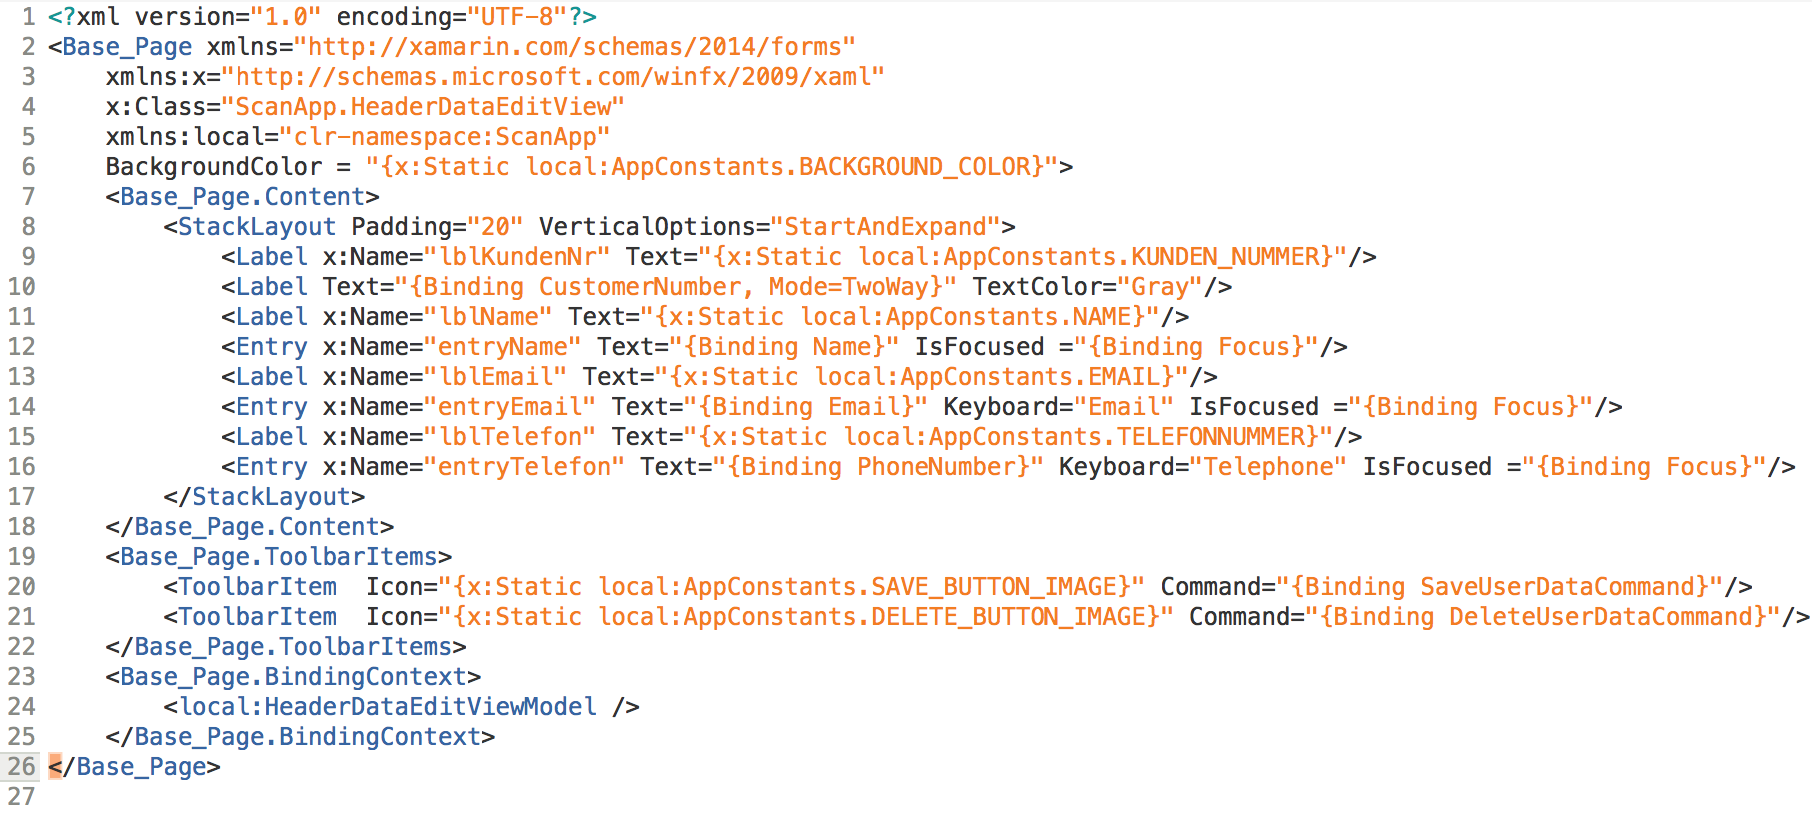
\includegraphics[scale = 0.435]{graphics/Typische_Xaml_Datei.png}
\caption{Typische Xaml-Datei}
\label{fig:abb23}
\end{figure}
\\Eine der wichtigsten Klassenvariablen der Klasse Xamarin.Forms.Page ist das Property
\textit{BindingContext}.
Mithilfe dieser Eigenschaft wird ein Viewmodel (in diesem Fall das HeaderDataEditViewModel) an der Page-Klasse gebunden (Siehe
\ref{fig:abb23}, Zeile 23-25).
\\In Zeile 12 findet eine typische Datenbindung ("`data binding"') statt.
Das Text-Property eines Entry-Textfeldes wird an das Property \textit{Name} gebunden, das im
Viewmodel definiert wird (siehe Abb.\ref{fig:abb33}).
Sobald der Text des Textfelds sich �ndert, wird das Viewmodel dar�ber informiert. Diese Bindung
funktioniert in beiden Richtungen, d.h. �nderungen, die im Viewmodel vorgenommen werden, werden in
der Ansicht angezeigt.\\In Abbildung \ref{fig:abb23}, Zeile 20 ist die Definition eines
Toolbarbuttons zu sehen. Sobald dieser Button gedr�ckt wird, wird ein Command ausgef�hrt, das an
das Property \textit{SaveUserDataCommand} des Viewmodels gebunden ist. D.h. dieses Klick-Event
l�st den Aufruf einer Methode in der Viewmodel-Klasse auf.
\\Durch das Attribut x:Name k�nnte man auf das Element aus der Code-Behind-Datei zugreifen und bspw.
den Text eines Labels oder die Textfarbe setzen.
% \\Das Ganze veranschaulicht, welche
% Vorteile das MVVM-Architekturmuster mit sich bringt.

\begin{figure}[!h]
\centering
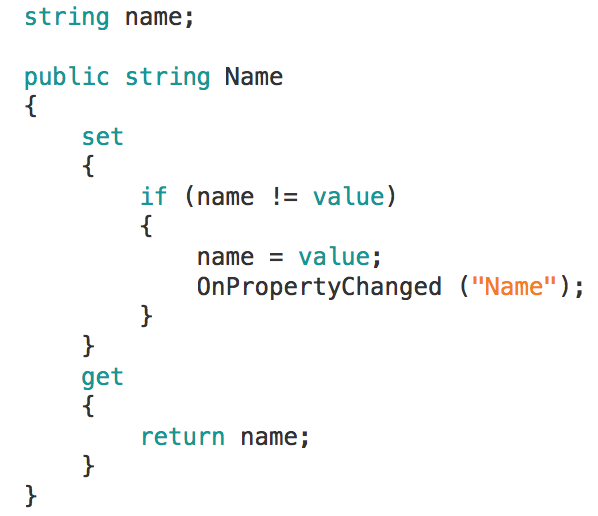
\includegraphics[scale = 0.6]{graphics/Bindable_Property.png}
\caption{Definition von Bindable Property}
\label{fig:abb33}
\end{figure}

\newpage
\subsection{Test}
Ein wichtiger Schritt im Entwicklungszyklus einer App ist das Testen. Es wird zwischen zwei Arten
von Tests unterschieden, UI- und Unit-Tests. 
W�hrend Unit-Tests die App-Logik testen, wird bei UI-Tests sichergestellt, dass die App so aussieht
und sich so verh�lt, wie man es erwartet, also es wird das Optische getestet.\\Ein typischer Weg,
eine App zu testen ist die zu starten und zu benutzen.
Im besten Fall tut die App genau das was sie tun soll - funktioniert korrekt und st�rzt nicht ab. Erfahrungsgem�� ist das so
gut wie nie der Fall. Diese Art von Testen, indem man die App auf einem realen Ger�t nutzt, wird als UI
Acceptance Testing bezeichnet.
Die zur Verf�gung gestellten Simulatoren erleichtern wesentlich den Testprozess, allerdings um
sicher zu gehen, dass eine App wirklich fehlerfrei funktioniert, kommt man an Tests auf reale Ger�te nicht
herum. Da es vor allem bei Android eine gro�e Vielfalt an Ger�ten gibt, kann das sehr m�hsam sein.
Softwarehersteller m�ssen nicht selten Apps auf dutzende sogar hunderte Ger�te installieren und
testen.\\Die meisten Developer verzichten auf systematisches Testen, weil die verf�gbaren Tools und
Dienste zu kompliziert und schwer zu benutzen sind und nur auf einem Ger�t bzw. Simulator ausgef�hrt
werden k�nnen. \\Abhilfe kann man sich bei einem Feature von Xamarin, genannt Xamarin Test Cloud,
schaffen.\\Alle Xamarin-Plattform-Abonnements beinhalten 60 Xamarin Test Cloud Ger�te-Minuten pro Monat. D.h. jeder Entwickler, der einen Xamarin Account hat,
kann die Dienste der Xamarin Test Cloud in Anspruch nehmen.
Xamarin verf�gt �ber 1600 reale iOS- und Android-Smartphones und Tabletts. An dieser Stelle muss
klargestellt werden, dass es allerdings nur iOS- und Android-Ger�te sind, also die Test Cloud von
Xamarin unterst�tzt noch nicht Windows Phone.
Mit der Test Cloud kann man leicht visuelle Inkonsistenzen feststellen, indem man die Ergebnisse eines UI-Tests auf
dutzende Ger�ten vergleicht. Der Entwickler hat die M�glichkeit Screenshots an beliebigen Stellen
des Tests zu machen.
Dar�ber hinaus bietet der Service auch Videoaufnahme von Tests.
Eine Ger�te-Minute wird konsumiert, wenn der Test auf einem Ger�t ausgef�hrt wird, wobei es keine
Rolle spielt ob die Tests parallel auf mehrere Ger�te oder nacheinander ausgef�hrt werden.

